\section{Delsystem}

Systemet är indelat i två olika delsystem. Dessa system kommer köras
sekvensiellt, alltså det ena efter det andra. Varje sekund kommer dessa två delsystem köras 10 gånger (dvs 10 cykler/sekund). Det första systemet kontrollerar
själva bilkörningen medan det andra systemet kontrollerar displayen. Se
figur~\ref{fig:system_diagram} för ett processchema.

\begin{figure}
  \centering
  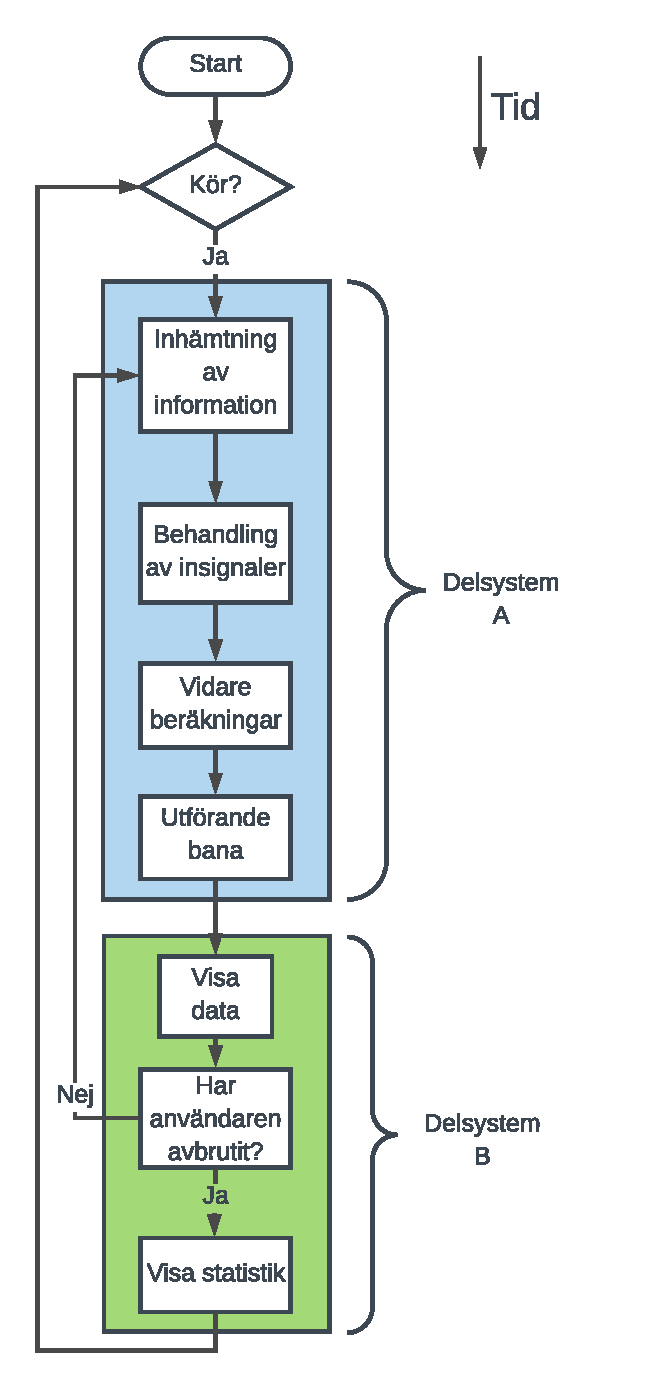
\includegraphics[width=\linewidth,height=0.9\textheight,keepaspectratio]{figures/Processchema.pdf}
  \caption{Processchema över systemets helhet.}%
  \label{fig:system_diagram}
\end{figure}

  \subsection{Delsystem A: Bana}
  
  Delsystem A är indelat i tre övergripande delar. I del A.1 hämtas all
  tillgänglig information in, i del A.2a görs beräkningar utifrån tillgänglig
  data, i del A.2b görs vidare beräkningar (alltså beräkningar som inte baseras
  direkt på den tillgängliga informationen), och i del A.3 utförs de ändringar
  som programmet bedömer är nödvändiga för att klara den valda varvtiden. 

    \subsubsection{Inhämtning av information}

    Information som finns tillgänglig är kraftigt begränsad. I praktiken kommer
    programmet endast fråga om någon av bilarna passerat en givare sedan
    programmet frågade förra gången.

    \subsubsection{Behandling av insignaler}

    De beräkningar som beror direkt på tillgänglig
    information. Då ny indata endast kommer då en bil passerar en givare görs dessa beräkningar inte varje cykel. 
 Ny indata används för att bestäma bilens position, starta en clocka och för att kalibrera en konstant. Dessa funktioner beskrivs 
mer ingående i \ref{sec:system_a_funcs}.

    \subsubsection{Vidare beräkningar}
    
    Den första beräkningen som görs är bilens nuvarande position. Detta görs med
    hjälp av en intern bild av banan och vetskapen om vilken hastighet och position bilen
    tidigare haft. Sedan beräknas den position som bäst gör att bilen klarar den satta
    varvtiden. För att räkna ut den beaktas enbart den nuvarande tiden och, om gemensam målgång är aktiverat, positionen av den andra bilen.  
I början av varvet görs  inte lika drastiska hastighetsändringar som mot slutet.

    Det sista som händer är att  informationen om bilens och banans skick används
    för att räkna ut vilket spänningspådrag som krävs för att få bilen att nå
    den hastighet och position som krävs.

    \subsubsection{Utförande}

    I utförandet skickas det nya spänningspådraget till banorna. 
	

    \subsubsection{Funktioner i delsystem A} \label{sec:system_a_funcs}
    I figur~\ref{fig:flow_diagram}  visas flödet av de funktioner som sker i delsystem A under en cykel.
    Här listas namn på funktionerna och deras funktion:
    \begin{itemize}
	\item old\textunderscore v: Lagring av bilens hastighet från segment, varv och tidigare lopp. Från denna databas kan andra funktioner få information om hur fort bilen tidigare har åkt. 	\item old\textunderscore position: Lagring av gammal data för bilens placering. Från denna databas kan andra funktioner få information om var bilen var förra cykeln, var bilen var för ett varv sedan m.m.
      \item indata: Avgör huruvida en givare har passerats sedan förra cykeln.

%car_constant
      \item car\textunderscore constant: car\textunderscore constant ska direkt påverka new\textunderscore u så att new\textunderscore u tillsammans med track\textunderscore u\textunderscore constant motsvarar den hastighet som anges av new\textunderscore v. car\textunderscore constant ändras endast vid ny indata, vilket innebär att den är konstant under resterande cykler. Genom att jämföra position med indatan kan programmet räkna ut felmarginalen som har uppstått och kalibreras så att man med större precision kan justera new\textunderscore u.
 
      \item position: Programmet räknar ut var på banan bilen befinner sig genom att hämta senaste positionen old\textunderscore position och sedan addera sträckan bilen har färdats sedan dess senaste värde. Sträckan som bilen har färdats kan räknas ut genom S=V\textasteriskcentered (delta)T, där V = old\textunderscore v och (delta)T = tidskillnaden mellan senaste cykel. Om det finns ny indata denna cykel, så är positionen känd och denna data används istället för att utgå ifrån gammal.
      \item clock: Hur länge bilen har varit i det nuvarande segmentet och varvet.

      \item car\textunderscore position\textunderscore dif: Endast aktiv om gemensam målgång aktiverad. Jämför bilarnas position med varandra. Funktionen utgår ifrån respektive bils placering (från old\textunderscore position) och hastighet (från old\textunderscore v) 
och ger ett värde på placeringsskillnaden för en viss hastighet. Detta kommer
sedan användas för att sätta bilarnas nya hastighet. Värdet blir stort om skillnaden i placering är stor men justeras också efter hastigeten. Dvs om bilarna ligger långt ifrån varandra men åker ganska fort kommer inte värdet bli lika stort som om bilarna legat lika långt ifrån varandra men haft lägre hastighet. Värdet är positivt om bil 1 ligger före bil 2 och negativt om bil 2 ligger före bil 1. På så sätt kan nästa funktion avgöra vilken bil som ligger först.
Värdet används sedan för att beräkna nästa hastighet (new\textunderscore v) som kommer ökas eller minskas för att få bilarna att köra ikapp varandra. 

      \item target: Den varvtid som manuellt har satts innan programet startade.
      \item target dif: Differensen mellan den önskade tiden och positionen relativt till den faktiska tiden och positionen. Görs genom att subtrahera de önskade värdena med de faktiska värdena. 
 
      \item agressivness: Justerar hur stora ändringar som görs på new\textunderscore v. Vid början av ett varv finns det mycket tid kvar och new\textunderscore v kan ändras lite i taget istället för att göra stora förändringar direkt. Dessutom är det onödigt att göra stora ändringar om bilarna befinner sig ungefär där de bör vara. agressivness räknas ut via; clock,  hur mycket av varvtiden återstår, target\textunderscore dif, hur långt ifrån målet befinner sig bilen och om gemensam målgång är aktiv tar agresivness även hänsyn till car\textunderscore position\textunderscore dif,  hur långt avståndet mellan de två bilarna är. 

%u_constant_map
      \item u\textunderscore constant\textunderscore map: En kartläggning över banan och de spänningsnivåer som behöver sättas så att spänningen blir jämn. Detta eftersom att spänningstillförseln beter sig olika för olika delar av banan. Kartläggningen kommer bygga på det register med inlagrad data som tagits fram genom tester.
      \item target\textunderscore dif: Bilens position relativt till var den borde vara vid den nuvarande tiden.
      
\item track\textunderscore u\textunderscore constant: Detta ät det förbestämda spänningsvärdet för ett visst subsegment på banan. Värdet tas fram manuellt genom prövning och lagras i u \textunderscore constant \textunderscore map. Ur position tar track \textunderscore u \textunderscore constant fram rätt spänningsvärde. 
     
 \item speed\textunderscore map: En kartläggning över banan och hur över hur fort man kan köra i olika delar av banan. Kartläggningen kommer bygga på det register med inlagrad data som tagits fram genom tester.

      \item speed\textunderscore constant: Den förbestämda maxhastigheten för nuvarande subsegment. Värdet tas fram manuellt genom prövning och lagras i speed\textunderscore map. Ur position tar speed\textunderscore constant fram rätt hastighet. 

% new_v     
\item new\textunderscore v: Beräknar den hastighet som bilen ska få nästa cykel. Funktionen tar förra cykelns hastighet (old\textunderscore v) 
och lägger till eller tar bort lite beroende på hur långt ifrån målet som bilarna ligger (target\textunderscore dif) och, om gemensam
målgång är aktiverad, hur långt ifrån varandra bilarna är (car\textunderscore position\textunderscore dif). Funktionen beror 
också på agressivness, högre agressivness ger större skillnad mellan new\textunderscore v och old\textunderscore v medan ett lågt värde gör att new\textunderscore v 
inte kommer ändras särskillt mycket.
new\textunderscore v används sedan för att sätta
new\textunderscore u. Högre new\textunderscore v ger högre new\textunderscore u och lägre new\textunderscore v ger lägre\textunderscore u. 
	
\item new\textunderscore u: Beräknar den spänning som ska appliceras beroende på vilken hastighet new\textunderscore v anger. Ett högre new\textunderscore v innebär ett högre new\textunderscore u. De andra parametrarna som påverkar new\textunderscore u är car\textunderscore constant och track\textunderscore u\textunderscore constant, desto högre dessa värden dessa antar desto högre värde antar också new\textunderscore u. New\textunderscore u är programmets sista output, dess värde 0 till 127 är det gaspådrag som appliceras på bilen.
    \end{itemize}

    \begin{figure}
      \centering
      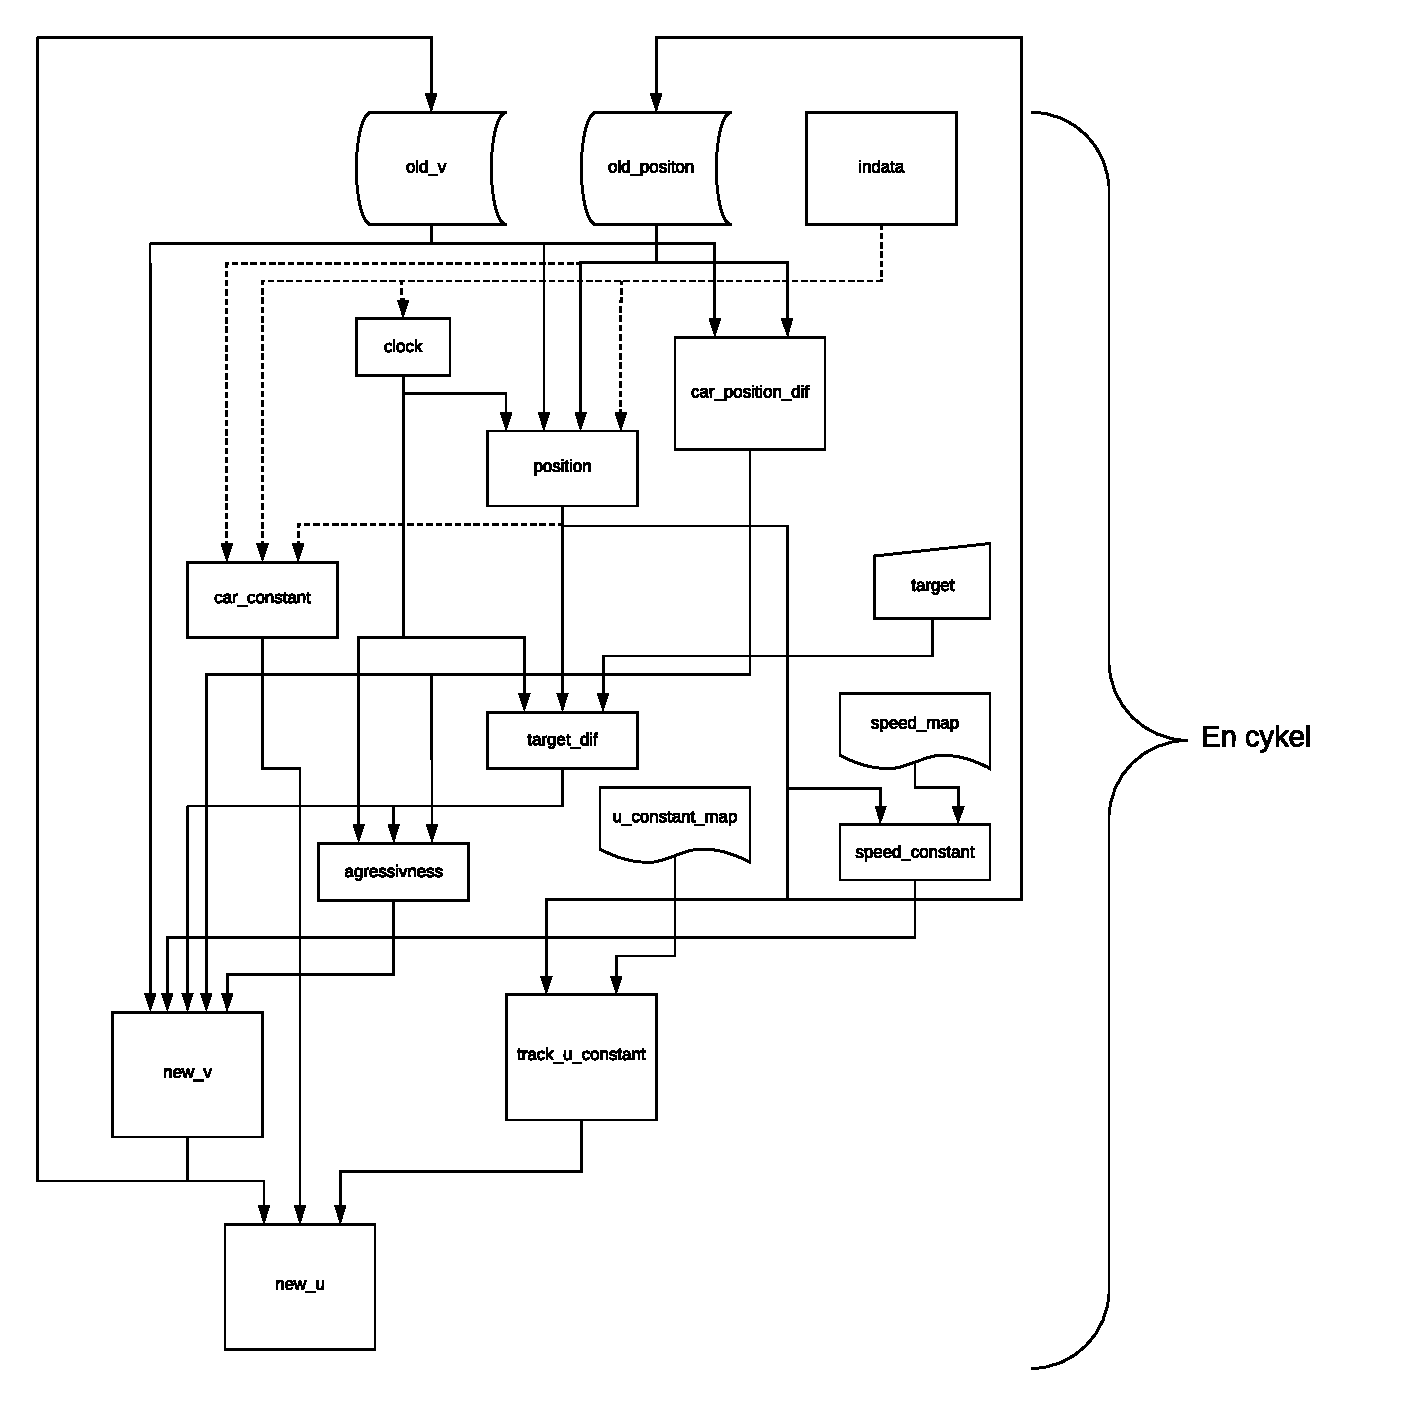
\includegraphics[width=\linewidth]{figures/flow.pdf}
      \caption{Funktionsflödet i delsystem A.}%
      \label{fig:flow_diagram}
    \end{figure}

  \subsection{Delsystem B: Display}

  Displayen ter sig enklare än delsystem A. Under körning ska, om ett nytt varv
  påbörjats, den senaste varvtiden och varvnumret skickas till displayen. Om
  stopp-knappen har tryckts ned ska systemet hoppa till resultat-skärmen och om
  inte så ska det fortsätta.

